\section{Related Work}

\begin{frame}
        \centering
        \huge Related Work
        \note{
                \begin{itemize}
                        \item a
                \end{itemize}
		}
\end{frame}

\begin{frame}
	\frametitle{Diffusion Prediction}
	\begin{columns}
		\begin{column}{0.5\textwidth}
			\begin{itemize}
				\item Susceptible-Infected framework
				\begin{itemize}
					\item Varies in how to reverse the process of diffusion to predict the source
				\end{itemize}
			\end{itemize}
		\end{column}
		\begin{column}{0.5\textwidth}
			\begin{figure}
				\centering
				\includegraphics[scale=0.45]{suceptible.png}
			\end{figure}
		\end{column}
	\end{columns}
	\note{
		As classically done in the field of diffusion modeling, existing approaches for
		source detection are based on the Susceptible-Infected framework defined on a
		given known graph of diffusion G = (U, E). When a user u in U becomes infected
		at time t, each neighbor v in the graph becomes infected at time t + du,v, with
		du,v being drawn from some delay distribution [4,5,16,19,20,22]. The various
		methods mainly differ in their way of reversing the process of diffusion to predict
		the most probable source when some infections are observed.
	}
\end{frame}

\begin{frame}
\frametitle{Rumor centrality}
	\begin{columns}
		\begin{column}{0.5\textwidth}
			\begin{itemize}
				\item Detecting sources of computer viruses in networks: theory and experiment
				\begin{itemize}
					\item Shah, D. and Zaman, T.
				\end{itemize}
			\end{itemize}
		\end{column}
		\begin{column}{0.5\textwidth}
			\begin{figure}
				\centering
				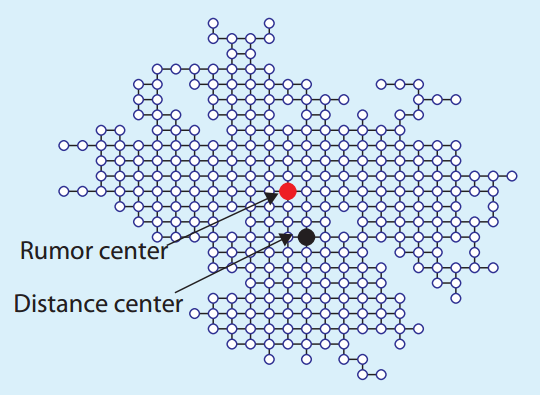
\includegraphics[scale=0.4]{rumor.png}
			\end{figure}
		\end{column}
	\end{columns}

	\footnotetext{Detecting sources of computer viruses in networks: theory and experiment by Shah, D., Zaman, T.}
	\note{
		The work of [20] was the first one to introduce the key concept of rumor
		centrality, a measure rendering the likelihood, for any content emitted from a node u in U, to spread over a given subset of infected users
	}
\end{frame}